\documentclass[9pt,twocolumn,twoside]{optica-suppl-materials}
\setboolean{shortarticle}{false}

\title{Netflix Architecture}

\author[]{Masand Nikita}
\author[]{Mentor: Prof. Pranav Nerurkar}

\affil[1]{Dept of Computer Engineering and IT, VJTI}

% To be edited by editor
% \dates{Compiled \today}


\begin{abstract}

\href{https://www.netflix.com/in/}{Netflix} was founded in 1997 by Marc Randolph and Reed Hastings in Scotts Valley, California and started with 30 employees with 925 working on pay-per-rent.Netflix, now the world’s leading Internet television network, has more than 69 million subscribers in 50 countries enjoying more than ten billion hours of TV shows and movies per month.At this scale, providing quality entertainment in a matter of a few seconds to every user is no joke. And as much as it means building top-notch infrastructure at a scale no other Internet service has done before, it also means that a lot of participants in the experience have to be negotiated with and kept satiated — from production companies supplying the content, to internet providers dealing with the network traffic Netflix brings upon them. They are very transparent and publish a lot of information online. This manuscript includes an in-depth information, research on the working of Netflix that makes it all the more interesting. The two major components or concepts that contribute to Netflix's success are microservices and chaos monkey. 

\end{abstract}
\setboolean{displaycopyright}{false} 

\begin{document}

\maketitle

\section{Why Netflix is not a Monolithic architecture? And what is monolithic?}
We assume that the Maps app on our phone tracks our location all the time and saves complex information about everywhere we go in a file, locations.txt. And we end up creating an app called LocoList, that looks for this locations.txt file and shows all the places recorded in that file in a simple list. It works flawlessly. Let’s say that developers of the Maps app realise it’s a better idea to store all our location information somewhere else than in that locations.txt file, and update the app so that it no longer creates or stores that file on our phone. And now LocoList can’t seem to find that locations.txt file it depended on for all its data, and there’s no other way it can extract that information from the Maps app either. LocoList no longer works now!
All our work on LocoList has gone into the trash because a change was made to Maps that broke your app. And while it might not seem a big deal here, on a huge service like Netflix the entire application going down because a change was made to one part of it can not only ruin the experience for users, it also means that all other parts of the application have to be rewritten to accommodate that one tiny change we made to one part of the app. Such a structure is what we call a \textbf{monolithic architecture}.

\section{Era of microservices and Netflix}
Netflix ushered in a revolution around ten years ago by rewriting the applications that run the entire service to fit into a microservices architecture which means that each application, or microservice’s code and resources are its very own. It will not share any of it with any other app by nature. And when two applications do need to talk to each other, they use an application programming interface (API), a tightly-controlled set of rules that both programs can handle. Developers can now make many changes, small or huge, to each application as long as they ensure that it plays well with the API. And since the one program knows the other’s API properly, no change will break the exchange of information.
Netflix estimates that it uses around 700 microservices to control each of the many parts of what makes up the entire Netflix service: one microservice stores what all shows we watched, one deducts the monthly fee from our credit card, etc.
\begin{quote}
    Netflix engineers can make changes to any part of the application and can introduce new changes rapidly while ensuring that nothing else in the entire service breaks down.
\end{quote}

\subsection*{Importance of Microservices}

\begin{condenseditemize}
\item[] 100s of microservices
\item[] 1000s of daily production changes
\item[] 10,000s of instances
\item[] 100,000s of customer interactions/minutes
\item[] 1,000,000s of customers
\item[] 10,000,000,000s of hours streamed
\item[] 10s of operations engineers
\end{condenseditemize}

\section{Netflix's CDN-Content Delivery Network called Open Connect}
A CDN take the original website and the media content it contains, and copy it across hundreds of servers spread all over the world. So when we log in from Mumbai, instead of connecting to the main Netflix server in the United States it will load a ditto copy of it from a CDN server that is the closest to Mumbai. This greatly reduces the latency - the time taken between a request and a response, and everything loads really fast.A growing user base means they must deliver higher number of content at more locations while lowering costs and this led them to build their own CDN, called Open Connect.
Netflix strikes deals with internet service providers and provides them the red box you saw above at no cost. ISPs install these along with their servers. These Open Connect boxes download the Netflix library for their region from the main servers in the US — if there are multiple of them, each will rather store content that is more popular with Netflix users in a region to prioritise speed. So a rarely watched film might take time to load more than a common series. 

\section{System Architecture of Netflix}
\subsection{Design}
\begin{figure}[htbp]
\centering
\fbox{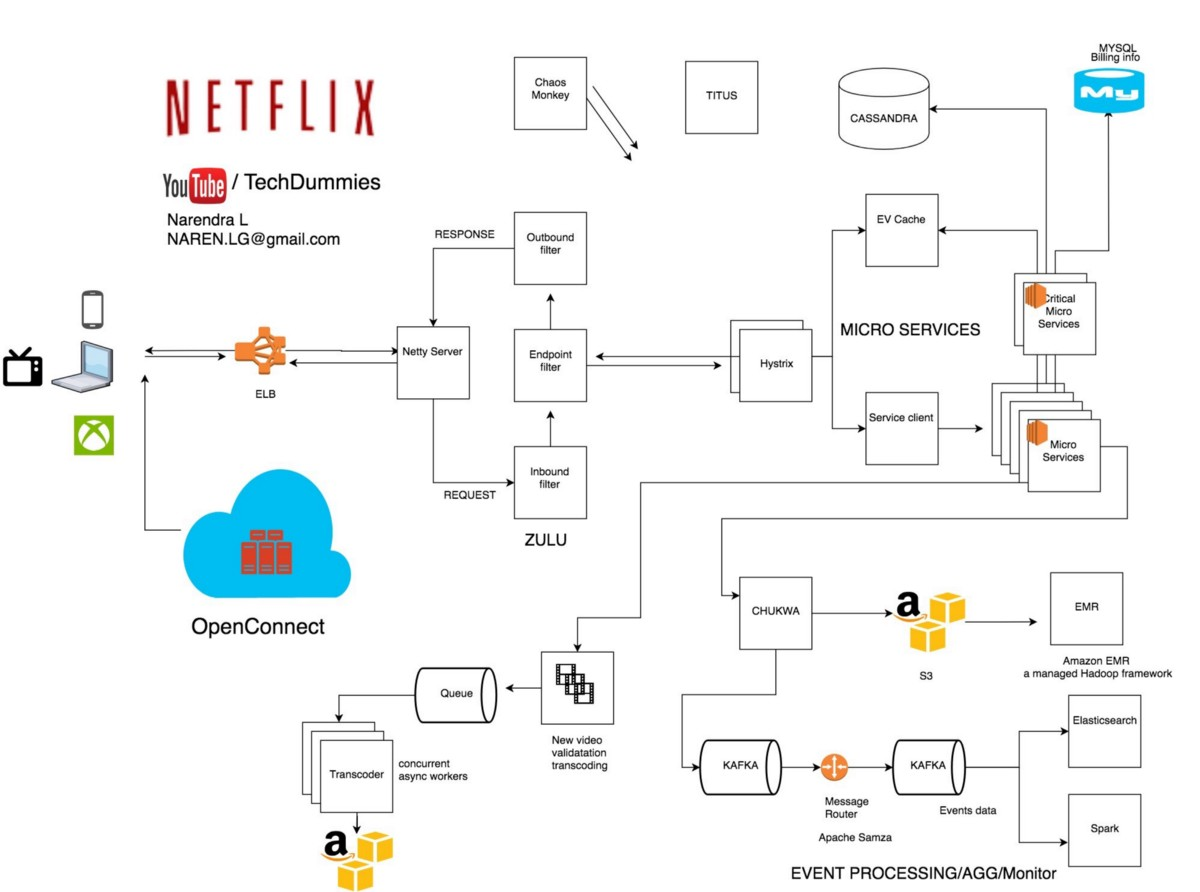
\includegraphics[width=\linewidth]{n2.jpg}}
\caption{Netflix : https://netflix.github.io/}
\label{fig:false-color}
\end{figure}

\subsection{Application and Data}
The Netflix culture of freedom and responsibility empowers engineers to craft solutions using whatever tools they feel are best suited to the task. In our experience, for a tool to be widely accepted, it must be compelling, add tremendous value, and reduce the overall cognitive load for the majority of Netflix engineers. Teams have the freedom to implement alternative solutions, but they also take on additional responsibility for maintaining these solutions. 
Table \ref{tab:stack} shows Netflix's technology stack

\begin{table}[htbp]
\centering
\caption{\bf Technology}
\label{stack}
\begin{tabular}{ccc}
\hline
Languages & Java, Python, JS \\
Database & MySQL, Cassandra, Oracle \\
CloudHosting & Amazon EC2 \\
JS UI Library & React \\
SQL Database-as-a-service & Amazon RDS \\
SQL Database-as-a-service & Amazon RDS \\
NoSQL Database-as-a-service & Amazon DynamoDB\\
Database Cluster Management & Dynomite\\
\hline
\end{tabular}
  \label{tab:shape-functions}
\end{table}

\section*{Hystrix}
Hystrix is a latency and fault tolerance library designed to isolate points of access to remote systems, services, and 3rd party libraries, stop cascading failure and enable resilience in complex distributed systems where failure is inevitable
\begin{figure}[htbp]
\centering
\fbox{
\includegraphics[width=\linewidth]{n3.jpg}}
\caption{Netflix : https://netflix.github.io/}
\label{fig:false-color}
\end{figure}
\section*{Chaos Monkey}
Any change to the production environment changes the resilience of the system. At Netflix, our production environment might see many hundreds of deploys every day. As a result, our confidence in an experimental result quickly diminishes with time.
\begin{figure}[htbp]
\centering
\fbox{
\includegraphics[width=\linewidth]{n6.jpeg}}
\caption{Netflix: https://devops.stackexchange.com/who-is-this-chaos-monkey}
\label{fig:false-color}
\end{figure}
In order to have experiments run unsupervised, we had to make them safe. We designed a circuit breaker for the experiment that would automatically end the experiment if we exceeded a predefined error budget. 
ChAP generates emails like the following:
\begin{quote}
    “We ran a ChAP canary which verifies that the [service in question] fallback path works (crucial for our availability) and it successfully caught an issue in the fallback path and the issue was resolved before it resulted in any availability incident!”
-a stunning Netflix colleague
\end{quote}
Chaos Monkey is a service which identifies groups of systems and randomly terminates one of the systems in a group. The service operates at a controlled time (does not run on weekends and holidays) and interval (only operates during business hours). In most cases we have designed our applications to continue working when a peer goes offline, but in those special cases we want to make sure there are people around to resolve and learn from any problems. With this in mind Chaos Monkey only runs in business hours with the intent that engineers will be alert and able to respond.
\section*{Netflix's image algorithm}
The new image algorithm, though, works in real time to project the image it thinks we'll respond to, and continues collecting data to improve its performance. And it's doing the same for 100 million other subscribers, collecting THAT information for further customization. 
\begin{figure}[htbp]
\centering
\fbox{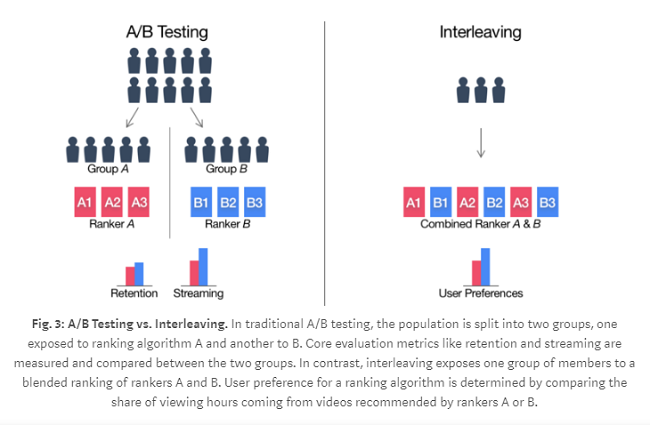
\includegraphics[width=\linewidth]{n5.png}}
\caption{Netflix https://medium.com/@NetflixTechBlog}
\label{fig:false-color}
\end{figure}
In the end, we get an image that Netflix's algorithm thinks will entice us to watch, but the key is that the picture could change tomorrow as the system "learns" more about us and subscribers like us. For any given show, there might be a dozen possible images loaded, which are ranked according to context. 


\begin{thebibliography}{}
\bibitem{}https://hackernoon.com/building-fault-tolerant-microservices-using-netflixs-hystrix-c36083ca9af5?sk=
\bibitem{}https://medium.com/refraction-tech-everything/how-netflix-works-the-hugely-simplified-complex-stuff-that-happens-every-time-you-hit-play-3a40c9be254b
\bibitem{}https://medium.com/@narengowda/netflix-system-design-dbec30fede8d
\bibitem{}http://highscalability.com/blog/2015/11/9/a-360-degree-view-of-the-entire-netflix-stack.html
\bibitem{}https://en.wikipedia.org/wiki/Netflix
\bibitem{}http://https://www.nginx.com/blog/microservices-at-netflix-architectural-best-practices/
\bibitem{}http://https://medium.com/netflix-techblog
\bibitem{}http://https://medium.com/netflix-techblog/how-we-build-code-at-netflix-c5d9bd727f15
\bibitem{}https://github.com/Netflix/SimianArmy/wiki/Chaos-Monkey
\bibitem{}https://medium.com/netflix-techblog/chap-chaos-automation-platform-53e6d528371f

\end{thebibliography}

\end{document}